\documentclass{article}

% if you need to pass options to natbib, use, e.g.:
%     \PassOptionsToPackage{numbers, compress}{natbib}
% before loading neurips_2021

% ready for submission

\PassOptionsToPackage{numbers, square}{natbib}
\usepackage{neurips_2021}

% to compile a preprint version, e.g., for submission to arXiv, add add the
% [preprint] option:
%     \usepackage[preprint]{neurips_2021}

% to compile a camera-ready version, add the [final] option, e.g.:https://www.overleaf.com/project/5f05abd2e41db100011026fc
%     \usepackage[final]{neurips_2021}

% to avoid loading the natbib package, add option nonatbib:
%    \usepackage[nonatbib]{neurips_2021}

\usepackage[utf8]{inputenc} % allow utf-8 input
\usepackage[T1]{fontenc}    % use 8-bit T1 fonts
\usepackage{hyperref}       % hyperlinks
\usepackage{url}            % simple URL typesetting
\usepackage{booktabs}       % professional-quality tables
\usepackage{amsfonts}       % blackboard math symbols
\usepackage{nicefrac}       % compact symbols for 1/2, etc.
\usepackage{microtype}      % microtypography
\usepackage{xcolor}         % colors


\usepackage{amssymb, bm, blkarray, multicol}
\usepackage{listings,lmodern}
\usepackage{graphicx}
\usepackage{enumitem}
\usepackage{algorithm}
\usepackage{algpseudocode}
\usepackage[nottoc]{tocbibind}
\usepackage{upgreek}

\usepackage{tikz}

\usepackage{mathtools}
\mathtoolsset{showonlyrefs}

\usepackage{latexsym}

\usepackage{physics} 

\newtheorem{theorem}{THEOREM}
\newtheorem{lemma}[theorem]{LEMMA}
\newtheorem{corollary}[theorem]{COROLLARY}
\newtheorem{proposition}[theorem]{PROPOSITION}
\newtheorem{remark}[theorem]{REMARK}
\newtheorem{definition}[theorem]{DEFINITION}
\newtheorem{fact}[theorem]{FACT}

\newtheorem{problem}[theorem]{PROBLEM}
\newtheorem{exercise}[theorem]{EXERCISE}
\def \set#1{\{#1\} }

\newcommand{\E}{\mathbb{E}}
\renewcommand{\var}{\mathrm{Var}}
\newcommand{\cov}{\mathrm{Cov}}
\newcommand{\KL}{\mathrm{KL}}
\newcommand{\neighb}{\text{ne}}
% \DeclareMathOperator*{\argmax}{arg\,max}
% \DeclareMathOperator*{\argmin}{arg\,min}
\newcommand{\Perp}{\mathrel{\text{\scalebox{1.07}{$\perp\mkern-10mu\perp$}}}}
\newcommand{\tildepi}{\tilde{\pi}}
\newcommand{\argdot}{{\,\vcenter{\hbox{\tiny$\bullet$}}\,}}%
% for comments
\newcommand{\hksay}[1]{[\textcolor{green!70!black}{\textbf{HK: }}\textcolor{green!50!black}{#1}]}
\newcommand{\ajsay}[1]{[\textcolor{red!70!black}{\textbf{AJ: }}\textcolor{red!50!black}{#1}]}

\renewcommand{\bibname}{References}
\global\long\def\given{\vert}%
\bibliographystyle{apalike}

\title{Kernel Tests for Markov Chain Monte Carlo}

% The \author macro works with any number of authors. There are two commands
% used to separate the names and addresses of multiple authors: \And and \AND.
%
% Using \And between authors leaves it to LaTeX to determine where to break the
% lines. Using \AND forces a line break at that point. So, if LaTeX puts 3 of 4
% authors names on the first line, and the last on the second line, try using
% \AND instead of \And before the third author name.

\author{%
  David S.~Hippocampus\thanks{Use footnote for providing further information
    about author (webpage, alternative address)---\emph{not} for acknowledging
    funding agencies.} \\
  Department of Computer Science\\
  Cranberry-Lemon University\\
  Pittsburgh, PA 15213 \\
  \texttt{hippo@cs.cranberry-lemon.edu} \\
  % examples of more authors
  % \And
  % Coauthor \\
  % Affiliation \\
  % Address \\
  % \texttt{email} \\
  % \AND
  % Coauthor \\
  % Affiliation \\
  % Address \\
  % \texttt{email} \\
  % \And
  % Coauthor \\
  % Affiliation \\
  % Address \\
  % \texttt{email} \\
  % \And
  % Coauthor \\
  % Affiliation \\
  % Address \\
  % \texttt{email} \\
}

\begin{document}

\maketitle

\begin{abstract}
    The Geweke diagnostic is a popular technique that assesses whether a Markov chain
  algorithm samples a posterior correctly: It
  generates samples from a joint distribution in two ways,
  one that involves the sampler and one that does not, and compares
  the two using a hypothesis test. 
%   It is popular with practitioners,
  It can in principle detect any type of error---lack of
  convergence, but also implementation errors, derivation errors, or
  insufficient lag. A practical limitation is the requisite
  two-sample test: For multivariate distributions on Euclidean space, the method typically compares a list of test statistics, such as first and second moments.
  It can be difficult to apply in machine learning, where spaces are not necessarily  
  Euclidean (e.g., graphs, text) and the distinction
  between parameters and latent variables blurs. 
  To broaden the method's scope, we cast the test as a sample  estimate of a probability metric, which we implement as maximum mean discrepancy (MMD). 
  The resulting test is nonparametric,
  benefits from the kernel trick to compute the metric without
  optimization, can be applied on any domain by plugging in a suitable
  kernel, and lets users draw on a large arsenal of established
  results to select a kernel. 
%   and interpret outcomes. 
  In experiments, we showcase its performance on a variety of problems involving plausible implementation mistakes.
%   We demonstrate its performance on non-Euclidean domains,
%   such as graphs, and show that it performs competitively even in the Euclidean case, albeit at
%   higher computational cost than some available alternatives.
\end{abstract}

\section{Introduction}
\label{section:intro}

Consider an unobserved
random variable $\Theta$ (a Bayesian model parameter, or a latent variable)
an observed random variable $X$, and a task involving the
posterior distribution of $\Theta$ given $X$. If the posterior cannot
be calculated analytically, Markov chain Monte Carlo sampling
(MCMC) is often the method of choice.
The Geweke diagnostic \cite{geweke_getting_2004} attempts to determine
whether the algorithm generates samples from the correct distribution.
That is not quite the same as a convergence diagnostic: The posterior
may be incorrect because the sampler has not yet converged---which is
what a convergence diagnostic tries to rule out---but also for a
variety of other reasons, such as 
implementation mistakes, errors or wrong assumptions in the
derivation, or because samples are collected from the chain too
frequently and introduce sequential dependence.
We refer to \citep{Robert:Casella} for more on MCMC, and on
convergence diagnostics.

Geweke's approach is simple and ingenious:
Assume a model with 
likelihood $p(x|\theta)$, prior density $\pi(\theta)$, and posterior
$\pi(\theta|x)$. The MCMC algorithm generates samples from an
approximate posterior $\tilde{\pi}(\theta|x)$. Our goal is to 
determine whether whether $\tilde{\pi}(\theta|x)=\pi(\theta|x)$. 
Since $p(x|\theta)$ and $\pi(\theta)$ are known, one can generate
samples from the exact joint distribution of $(X,\Theta)$ as
\begin{equation*}
  \Theta_i\sim \pi
  \quad\text{ and }\quad
  X_i\sim(\argdot|\Theta_i)\quad\text{ for }i=1,\ldots,n\;.
\end{equation*}
Call this the \emph{forward factorization} of the joint distribution.
Alternatively, one can use the \emph{backward factorization}
\begin{equation*}
  X'_i\sim p(\argdot)=\int p(\argdot|\theta)\pi(\theta)d\theta
  \quad\text{ and }\quad
  \Theta'_i\sim\tilde{\pi}(\argdot|X'_i)\;.
\end{equation*}
(Note $X'_i$ can be generated by drawing a pair, say $(X_i',\Theta_i'')$, from the forward joint,
and discarding $\Theta_i''$.) The sampler is correct if (and only if) ${(X_1,\Theta_1),\ldots,(X_n,\Theta_n)}$
and ${(X_1',\Theta_1'),\ldots,(X_n',\Theta_n')}$ have the same
distribution. Whether that is the case is determined using a
hypothesis test.

There is no free lunch: The approximate posterior
$\tilde{\pi}(\argdot|X_i)$ in the backward factorization
is represented by the sampler, which must burn in for \emph{each}
value of $X_i$, so arguably, properly using the diagnostic requires a
diagnostic. Letting the sampler burn in separately for each $X_i$ is
costly; starting with a previous value in the hope of reducing burn-in
is possible, but turns the diagnostic as a whole into a Markov chain
(and technically speaking into a Gibbs sampler), which must converge.
See Section \ref{related:work} for references on the problem, and on
mitigation strategies.
Nonetheless, Geweke's method has proven useful in practice, and can pick up
on suprisingly subtle mistakes.
It has been invoked, for example, by \citet{del_negro_time_2015} and
\citet{karlsson_corrigendum_2017} to correct two highly cited MCMC
algorithms in the econometrics literature, over a decade after their
initial publications.
As noted by \citet{grosse_testing_2014}, one may easily check that each of the sampler's steps preserves detailed balance, but a few errors may still slip through. 
In our own experience, it is often the detection of coding-,
derivation-, and other forms of ``human error'' where the Geweke diagnostic really
shines, and we would argue that it should be used as a complement to
mixing diagnostics, not as a replacement.

\textcolor{red}{remainder of section 1: One (short) paragraph
  summarizing what we do}


% % Markov chain Monte Carlo (MCMC) is an indispensable tool in modern Bayesian analysis, where a great majority of models have intractable posteriors and require simulation.
% Suppose we are faced with a Bayesian inference problem. 
% We model observed data $\bar{y}$ with a model $p(y|\theta)$, which is parameterized by $\theta\in \Theta$. 
% Given our observations, we wish to update our prior belief $\pi(\theta)$ and compute the posterior $\pi(\theta|y)=p(y|\theta)\pi(\theta)/p(y)$. 
% \footnote{For simplicity, we consider only probability distributions specified by densities with respect to the Lebesgue measure, and the extension to general measures is a routine.} 
% Apart from simple models, calculating the normalizer $p(y)=\int p(y\given \theta) \pi(\theta) \dd \theta$ is intractable, and the posterior is not given in closed form.
% Instead, we simulate the posterior by drawing samples from a Markov Chain with $\pi(\theta|y)$ as its stationary distribution using a Markov Chain Monte Carlo (MCMC) algorithm  \citep{metropolis_equation_1953}. Since valid inference requires the eponymous Markov chain to have converged to its stationary distribution, we apply one of the many convergence diagnostics in the literature \citep{cowles_markov_1996} to our samples and proceed. 

% However, there is a chance that the algorithm has been implemented incorrectly and the chain has converged to the wrong distribution. If undetected, the errors may even propagate through the literature. For example, \cite{del_negro_time_2015} and \cite{karlsson_corrigendum_2017} correct two highly cited MCMC algorithms in the econometrics literature --- over a decade after their initial publications. Principled methods for diagnosing these mistakes are thus quite useful. As noted by \cite{grosse_testing_2014}, one may easily check that each of the sampler's steps preserves detailed balance, but a few errors may still slip through. We must validate the behavior of the entire sampler to have full confidence in the results.

% MCMC methods are stochastic, which means we are limited to validating statistical properties of their outputs. Yet the form of the posterior is typically unknown, and quantities characterizing the distribution (e.g., mean and variance) unavailable. An ingenious solution proposed by \citet{geweke_getting_2004} is to examine a consistency property that the true posterior distribution should satisfy. 
% A Bayesian model defined by a likelihood $p(y\given \theta)$ and a prior $\pi(\theta)$ defines a joint distribution of $y$ and $\theta$, which follows $p(y\given \theta) \pi(\theta) = \pi(\theta\given y) p(y)$. Thus, a tractable alternative $\tilde{\pi}(\theta\given y)$ to the posterior should satisfy 
% \begin{equation}
%     p(y\given \theta) \pi(\theta) = \tilde{\pi}(\theta\given y) p(y)
%     \label{eq:joint}
% \end{equation}

% Crucially, this relation can be empirically tested.
% Let us call the left-side factorization the forward joint and the right the backward joint. If $\tilde{\pi}(\theta\given y)$ is correct, samples from either should be statistically indistinguishable. The Geweke test formalizes this idea. First, samples from the forward and backward joints are drawn. A set of statistical hypothesis tests then check for the equality of the expectations of \textit{test functions} across both sets --- for example, all empirical first and second moments. After correcting for multiple testing, if any individual null hypothesis is rejected, the implementation is likely flawed.
% % If the implementation is correct, then the Geweke test has a high probability of failing to reject the null. 
% This approach, however, will be unable to detect errors in the posterior sampler that lead to discrepancies outside of the given test functions; for example, in higher moments or the dependency between $y$ and $\theta$.

% We address this shortcoming by introducing two two-sample tests based on Maximum Mean Discrepancy \citep{gretton_kernel_2012} that can be viewed as kernel-based extensions of the Geweke test and other methods. The tests are nonparametric and do not require manual specification of test functions; given the right kernel, they can detect any error in an MCMC algorithm. The tests perform competitively with existing alternatives in a variety of settings, though they are quadratic in the number of samples compared to linear or log-linear for alternative tests. We show that kernel choice and the inclusion of hand-picked features relevant to MCMC can dramatically improve test power. In addition, the MMD tests more easily generalize to domains other than the Euclidean space $\mathbb{R}^{d}$ ($d\geq 1)$. We hope they will enable researchers to be more confident in publishing their own results as well as building on existing ones.

\section{Background: the MMD two-sample test (AND Geweke test...?)} 

To implement the Geweke test, one has to decide whether samples from the forward
and backward joints follow the same distribution. That is usually done as
follows: Consider more generally two 
random quantities $X$ and $Z$, with distributions $P$ and $Q$.
Given i.i.d.\ samples
${X_1,\ldots,X_n\sim P}$ and ${Z_1,\ldots,Z_n\sim Q}$, we must decide
whether or not $P=Q$ holds.
We denote the sample estimates of the expectations of a real-valued
function $f$ as
\begin{equation*}
  \hat{\mathbb{E}}[f(X)]\;:=\;\frac{1}{n}\sum_{i\leq n}f(X_i)\;
  \quad\text{ and }\quad
  \hat{\mathbb{E}}[f(Z)]\;:=\;\frac{1}{n}\sum_{i\leq n}f(Z_i)\;.
\end{equation*}
To compare distributions, choose a list of real-valued test functions
${t_1,\ldots,t_k}$, and define
\begin{equation*}
  T_{\text{max}}\;:=\;\max_{j\leq k}|\hat{\mathbb{E}}[t_j(X)]-\hat{\mathbb{E}}[t_j(Z)]|\;.
\end{equation*}
Given an accuracy ${c>0}$, distributions are then compared 
according to the rule
\begin{equation*}
  \text{ decide }X \text{ and } Z \text{ have distinct distributions }
  \quad\Longleftrightarrow\quad
  T_{\text{max}}\geq c\;.
\end{equation*}
\citet{geweke_getting_2004}, for example, chooses the functions
$t_j$ such that their expectations are first and second moments (where
the covariance matrix is approximated by a few leading eigenvalues).
In the parlance of statistics, the procedure above is a two-sample
hypothesis test, with test statistic $T_{\text{max}}$, null hypothesis
${P=Q}$, and alternative ${P\neq Q}$. The choice of $c$
calibrates between type I errors (falsely deciding that ${P\neq
  Q}$),
and type II errors (deciding ${P=Q}$ when distributions differ). In
terms of the Geweke diagnostic, a type II error would lead us to
believe that an incorrect sampler is correct.

To generalize this approach, let $\mathcal{F}$ be an arbitrary
(possibly infinite) class of real-valued functions, and consider the quantity
\begin{equation*}
  d_{\mathcal{F}}(X,Z)\;:=\;\sup_{f\in\mathcal{F}}|\mathbb{E}[f(X)]-\mathbb{E}[f(Z)]|\;.
\end{equation*}
One way to interpret $d_\mathcal{F}$ is as a test statistic: 
The sample estimate
\begin{equation}
  \hat{d}_\mathcal{F}(X,Z)\;:=\;
  \sup_{f\in\mathcal{F}}|\hat{\mathbb{E}}[f(X)]-\hat{\mathbb{E}}[f(X)]| \label{eq:naive-IPM}
\end{equation}
defines a hypothesis test with decision rule 
${\hat{d}_\mathcal{F}(X,Z)\geq\alpha}$. Clearly, choosing
$\mathcal{F}$ as ${\{t_1,\ldots,t_k\}}$ recovers ${\hat{d}_\mathcal{F}(X,Z)=T_{\text{max}}}$.
Another interpretation is as a distance between distributions:
If $\mathcal{F}$ is sufficiently large, $d_\mathcal{F}$ defines a
metric on probability measures. Metrics of this form are called
\emph{integral probability metrics}. Examples are the Wasserstein
distance of order 1 (choose $\mathcal{F}$ as all Lipschitz functions
with constant 1), the total variation distance ($\mathcal{F}$ consists
of all indicator functions of measurable sets), or, on the real line,
the Kolmogorov-Smirnov distance (use the indicators of
all sets of the form ${(-\infty,x]}$). See \cite{mueller:1997} for an overview.

Our objective is to choose $\mathcal{F}$ so that the resulting test is
(i) accurate, (ii) applicable on a range of
domains and (iii) practically feasible.
Accuracy depends on the choice of $\mathcal{F}$.
Statistics distinguishes between \emph{parametric} tests,
where $\mathcal{F}$ is finite, and \emph{nonparametric} tests, where it is
infinite. Thus, the Geweke diagnostic uses a parametric test.
Such tests have some fundamental limitations: It is not hard to
verify, for example, that $d_\mathcal{F}$ is not positive definite if
$\mathcal{F}$ is finite (unless the domain is a finite set, or one
restricts to a very small subset of distributions), so one cannot
conclude from ${d_\mathcal{F}(X,Z)=0}$ that $X$ and $Z$ are
identically distributed. Thus, even in the limit of infinite sample
size, every parametric test will produce type
II errors for certain pairs of distributions.
This problem does not arise if we choose a function class that makes
$d_{\mathcal{F}}$ a metric---if so,
${d_\mathcal{F}(X,Z)=0}$ indeed guarantees $X$ and $Z$ are identically
distributed.
None of the metrics above yields a feasible test, however, since
the supremum over the infinite class $\mathcal{F}$ cannot be evaluated.

A nonparametric yet computable test
can be obtained as follows: Fix a reproducing kernel
Hilbert space $\mathcal{H}$, with kernel
${k:\mathcal{X}\times\mathcal{X}\rightarrow\mathbb{R}}$, and 
choose $\mathcal{F}$ as the unit ball ${B(\mathcal{H})}$ in $\mathcal{H}$.
\begin{equation*}
  \mathrm{MMD}(P,Q)
  \;:=\;
  d_{B(\mathcal{H})}(X,Z)
  \;=\;
  \sup_{f\in B(\mathcal{H})}|\mathbb{E}[f(X)]-\mathbb{E}[f(Z)]|
\end{equation*}
is called the \emph{maximum mean discrepancy} of $P$ and $Q$.
One can show that this is a metric if $k$ has suitable properties---if it is a
so-called \emph{characteristic kernel} \citep{fukumizu_kernel_2007}. 
The definition still involves a supremum over an infinite class
$\mathcal{F}$, but one can also show that
\begin{equation}
  \mathrm{MMD}(P,Q)^2\;=\;\mathbb{E}[k(X,X')]-2\mathbb{E}[k(X,Z)]+\mathbb{E}[k(Z,Z')]\;,\label{eq:mmd2}
\end{equation}
for four independent random variables ${X,X'\sim P}$ and ${Z,Z'\sim
  Q}$ \cite{gretton_kernel_2012}.
  
In contrast to the naive estimator \eqref{eq:naive-IPM}, the form in \eqref{eq:mmd2} allows estimation with pair-wise sample evaluations of the kernel. 
In particular, we can consider the following estimators, 
\begin{align}
        \widehat{\mathrm{MMD}^2}_{V} &\coloneqq \frac{1}{n^2}  \sum_{i,j=1}^n k\left(X_{i}, X_{j}\right)
        -\frac{2}{n^2} \sum_{i,j=1}^{n} k\left(X_{i}, \tilde{X}_{j}\right)+\frac{1}{n^2}\sum_{i,j=1}^{n} k\left(\tilde{X}_{i}, \tilde{X}_{j}\right), \label{eq:mmd_biased}\\
    \widehat{\mathrm{MMD}^2}_{U} &\coloneqq \frac{1}{{n\choose 2}} \sum_{1\leq i < j}^{n} k\left(X_{i}, X_{j}\right) -\frac{2}{n^2} \sum_{i,j = 1}^{n} k\left(X_{i}, \tilde{X}_{j}\right) + \frac{1}{{n \choose 2}}\sum_{1\leq i < j}^n k\left(\tilde{X}_{i}, \tilde{X}_{j}\right), \label{eq:mmd_unbiased}\\
\end{align}
which are, respectively, a V-statistic and a U-statistic \citep{Hoeffding1948, Vaart_1998, Mises1947asymptotic}.
Asymptotic behaviours of these estimators have been established, which enable us to calibrate a threshold to reject the null. 
% We reject the null hypothesis if a statistic $T_n$ (either of the above estimators) is sufficiently large. 
% In doing so, we need to control the type-I error rate (i.e., the probability of falsely rejecting the null). 
Specifically, with $T_n$ denoting either of the estimators \eqref{eq:mmd_biased}, \eqref{eq:mmd_unbiased}, we design a threshold $c_{\alpha, n}$ such that the type-I error $\mathrm{Prob} (T_n > c_{\alpha, n}\given H_0)\leq \alpha$ is bounded by a given significance level $\alpha \in (0,1)$.
% The asymptotic distributions of the statistics in \eqref{eq:mmd_biased} and \eqref{eq:mmd_unbiased} have been studied. 
If the samples are i.i.d., we can simulate the distribution under the null $H_0: P=\tilde{P}$ by repeatedly permuting the samples and taking as the test threshold the $1-\alpha$ empirical quantile of the bootstrapped statistics \citep{gretton_kernel_2012}. 
When the samples are not i.i.d., as in the case of Markov chains, the permutation bootstrap is inappropriate because it breaks the independence between observations.
\citet{chwialkowski_wild_2014} provide a bootstrap procedure for the V-statistic \eqref{eq:mmd_biased} with correlated samples ($\tau$-mixing processes).
In this case, we can simulate the null distribution by drawing the wild-bootstrapped MMD
\begin{equation}
\begin{array}{c}
\widehat{\mathrm{MMD}^2}_{V, b}=\frac{1}{n^2} \sum_{i,j=1}^{n} W_{i}^{(x)} W_{j}^{(x)} k\left(X_{i}, X_{j}\right)+\frac{1}{n^2} \sum_{i,j=1}^{n} W_{i}^{(y)} W_{j}^{(y)} k\left(\tilde{X}_{i}, \tilde{X}_{j}\right) \\
\quad-\frac{2}{n^2} \sum_{i,j=1}^{n}W_{i}^{(x)} W_{j}^{(y)} k\left(X_{i}, \tilde{X}_{j}\right)
\end{array}
\label{eq:wb_mmd}
\end{equation}
where $\{W_{t}^{(x)}\}_{t\leq n}$, $\{W_{t}^{(y)}\}_{t\leq n}$ are two wild bootstrap processes.
They are independent of each other and samples $\{X_1, \dots, X_n\},$ $\{Z_1, \dots, Z_n\}$, and follow $W_{t}=\exp(-1/l) W_{t-1}+\sqrt{1-\exp(-2/{l})}\epsilon_{t}$,
% \begin{equation}
%     W_{t}=\exp{\left(-\frac{1}{l}\right)} W_{t-1}+\sqrt{1-\exp{\left(-\frac{2}{l}\right)}} \epsilon_{t}
%     \label{eq:wb_process}
% \end{equation}
with $W_{0} \sim \mathcal{N}(0,1)$ and $\epsilon_{t} \sim \mathcal{N}(0,1)$ \cite[see, ][]{chwialkowski_wild_2014, leucht_dependent_2013}.

% Importantly, the MMD test is consistent in power against a fixed alternative; i.e., the type-II error converges to zero as the sample size increases.

\begin{table}[b]
    \caption{Backward Joint Sampling Algorithms. The symbol $L$ denotes the burn-in size, and $j$ is the thinning step size.
    The transition kernel of an MCMC sampler for the target $\tildepi(\theta\given y)$ is denoted by $q_{y}(\theta_{1} \given \theta_0)$ (density of the next position $\theta_1$ conditioned on the present $\theta_0$). 
    }
    \label{tab:sampling}
    \centering
    \begin{tabular}{l|l}
    \toprule
        Successive-conditional (SC) & Backward-conditional (BC) \\
    \midrule  
    
    Initialize $\theta_{0} \sim p(\theta)$                                      & Repeat: $\theta_{0} \sim p(\theta), y_{i} \sim p(y|\theta_{0})$ \\
    Repeat: $y_{i} \sim p(y|\theta_{i-1}), \theta_{i} \sim q_{y_i}(\theta|\theta_{i-1})$   & \qquad $\theta_{l} \sim q_{y_i}(\theta|\theta_{l-1})$ for $l=1,...,L+1$ \\
    Keep $\{(y_{i}, \theta_{i}) \given i=L+kj; k=1,2,\ldots; j\in\mathbb{N} \}$                     & \qquad Keep $(y_{i}, \theta_{L+1})$ \\
    \bottomrule
    \end{tabular}
\end{table}
\section{Kernel tests for MCMC}
Our objective is to check the consistency of the backward joint $\tildepi(\theta \given y) p(y)$, defined by an MCMC sampler for $\tildepi(\theta\given y)$, with the forward joint $p(y\given \theta)\pi(\theta).$
In this section, we introduce two versions of the MMD test, which differ in their sampling method for the backward joint.  
% Note that sampling from the the forward joint is straightforward by ancestral sampling: draw a parameter $\theta_0$ from the prior $\pi(\theta)$, and then a data point $y_0\sim p(y|\theta_0)$. 
% We therefore use the same sampling method for the forward joint, and consider two sampling algorithms for the backward: successive-conditional (SC) algorithm \citep{geweke_getting_2004} and backward-conditional (BC) algorithm \citep{gandy_unit_2020}. 

% In the following, we denote the transition kernel of an MCMC sampler for the target $\tildepi(\theta\given y)$ by $q_{y}(\theta_{1} \given \theta_0)$ (probability density of moving from $\theta_0$ to $\theta_1$). 
% In the following, we denote a sample from the forward joint by $S_f=\{(y_i, \theta_i)\}_{i=1}^n$.

% Like the Geweke test, our methods compare samples from the forward and backward joints in \eqref{eq:joint}.
% They share the same forward joint sampling algorithm, but differ in their choice of backward joint sampling algorithm and subsequent construction of the test threshold.

% The marginal-conditional (MC) algorithm samples from the forward joint by drawing parameters from the prior, followed by drawing data from the likelihood, conditioned on the sampled parameters.
% The samples are independent and the algorithm easily parallelized.

% There are two sampling methods for the backward joint.
% As described in \cite{geweke_getting_2004}, successive-conditional (SC) algorithm involves drawing sequentially from a Markov chain. The chain is initialized from the prior, then run forward by alternating draws from the likelihood, conditioned on the parameters, and the posterior MCMC sampler, conditioned on the data. A single sample is comprised of a draw from the likelihood and a draw from the posterior sampler. We may thin the successive-conditional samples to reduce their serial dependence and type I error rates. 



\subsection{Successive-conditional MMD Test}
We first consider the MMD test with the SC algorithm (Table \ref{tab:sampling}, left), termed the successive conditional MMD test (MMD-SC).  
% The successive-conditional MMD (MMD-SC) extends the the Geweke test. 
The SC algorithm involves drawing sequentially from a Markov chain. The chain is initialized from the prior, then run forward by alternating draws from the likelihood, conditioned on the parameters, and the posterior MCMC sampler, conditioned on the data. 
A single sample is comprised of a draw from the likelihood and a draw from the posterior sampler.
We may thin the successive-conditional samples to reduce their serial dependence and type-I error rates. 
Since the samples are correlated, we use the wild-bootstrapped MMD test from \cite{chwialkowski_wild_2014}. 

The testing procedure is given as follows. For significance level $\alpha$ and $B$ bootstrap samples, 
\begin{enumerate}
    \item Draw a forward-joint sample $S_f=\{(y_i,\theta_i)\}_{i=1}^n$ by ancestral sampling.
    \item Draw a backward-joint sample $S_{b}^{\mathrm{SC}}\{(\tilde{y}_i, \tilde{\theta}_{i})\}_{i=1}^{n}$ with the SC algorithm.
    % \item Apply test functions to both samples and normalize feature scales by their pooled standard deviation
    \item Calculate $\widehat{\mathrm{MMD}}_{V}^{2}$ using $S_f$ and $S_b^{\mathrm{SC}}$.
    \item Simulate $\{\widehat{\mathrm{MMD}}^{2}_{V, b}\}_{b=1}^{B}$ using \eqref{eq:wb_mmd} and calculate $c_{\alpha}$, their $1-\alpha$ empirical quantile.
    \item If $\widehat{\mathrm{MMD}}^{2}_{V} \geq c_{\alpha}$, reject the null hypothesis (suspect an error).
\end{enumerate}
For the wild bootstrap process, we set $l$ equal to $5\%$ of the sample size after thinning.

\subsection{Backward-conditional MMD Test}
The backward conditional MMD test (MMD-BC) uses the BC algorithm (Table \ref{tab:sampling}, right). 
The BC algorithm first draws from the (model) marginal of the data, burn in the MCMC sampler (conditioned on the generated data) and then obtain a parameter sample.
Since the samples are all independent, we can calculate the unbiased MMD statistic and use permutation bootstrapping to generate the test threshold as described in \cite{gretton_kernel_2012}. In contrast to the successive-conditional samples, the backwards-conditional samples can be drawn in parallel; the trade-off, however, is that each sample requires a burn-in period, while the successive-conditional samples require only one burn-in.

For a significance level $\alpha$ and $B$ bootstrap samples, the testing procedure is as follows.
\begin{enumerate}
    \item Draw a forward-joint sample $S_f=\{(y_i,\theta_i)\}_{i=1}^n$ by ancestral sampling.
    \item Draw a backward-joint sample $S_{b}^{\mathrm{BC}}\{(\tilde{y}_i, \tilde{\theta}_{i})\}_{i=1}^{n}$ with the BC algorithm.
    % \item Apply test functions to both samples and normalize scales by their pooled standard deviations
    \item Calculate $\widehat{\mathrm{MMD}}_{U}^{2}$ using $S_f$ and $S_b^{\mathrm{BC}}$.
    \item Simulate the null distribution of $\widehat{\mathrm{MMD}}_{U}^{2}$ via permutation and calculate the $1-\alpha$ empirical quantile $c_{\alpha}.$
    \item If $\widehat{\mathrm{MMD}}_{U}^{2} \geq c_{\alpha}$, reject the null hypothesis that the distributions are the same
\end{enumerate}

An additional advantage of the MMD-BC test is that it may provide some guidance in choosing the number of burn-in samples for inference; a correct sampler may still fail the test if $L$ is set too low.

\subsection{Kernel Selection}
While the MMD test is consistent for any characteristic kernel, the finite-sample performance of the test critically depends on the choice of the kernel. 
It is known that poor kernel choice leads to degrading test performance, particularly in high dimension. 
\cite{reddi_decreasing_2014} show this explicitly for the Gaussian and Laplace kernels, where a poor choice of the bandwidth parameter makes the population MMD extremely small, resulting in a challenging testing problem.
Note that as our tests operate on the product space of the data and parameter sets, the input dimension tends to be high.
Therefore, to improve the test's sensitivity, we need to construct a kernel that help capture the difference between the joint distributions.

In addition to the raw features $g(y, \theta)=[y,\theta]^\top,$ following \cite{gandy_unit_2020}, we use two additional features
\[h(y, \theta)=\begin{bmatrix}p(y|\theta), & \pi(\theta) \end{bmatrix}^{\top}\]
that is, the evaluations of the likelihood $p(y\given\theta)$ and the prior $\pi(\theta)$ on the sample.
As we will see in Section \ref{sec:experiments}, this simple heuristic is useful in our setting. 
Intuitively, under an incorrect posterior distribution, certain parameter values will be more or less likely to be observed than they would be under the correct posterior; since $\pi(\theta|y) \propto p(y\given \theta)\pi(\theta)$, these discrepancies should manifest in the likelihood and prior.

In addition to using handcrafted features as above, we can also consider optimizing a kernel to maximize (an estimate of) the test power, such as by choosing an optimal scale \citep{Gretton2012, Sutherland2017} or learning distinguishing features with deep neural networks \citep{Liu2020}. 
These approaches are subject to the reduced test data size caused by sample splitting and may result in power loss if the available data is limited.  
However, in our setting (MMD-BC), we can generate as many independent samples as needed, this issue does not arise. 
In our experiments, to establish a fair comparison, we only consider the features $g$ and $h$. 
Nonetheless, our practical recommendation is to additionally use the aforementioned techniques.
% we use the features (test functions)
% \begin{equation}
%     g(\theta, y) = \begin{bmatrix} y & \theta \end{bmatrix}^{\top} \quad h(\theta, y) = \begin{bmatrix}p(y|\theta)) & p(\theta) \end{bmatrix}^{\top}
%     \label{eq:testfn}
% \end{equation}

% While $g(\theta, y)$ are all that are required for consistency, the MMD tests still benefit from the inclusion of MCMC-specific test functions. 

% \hksay{We should move the following info to the experiment section.}
% Any characteristic kernel will provide a consistent test.
% However, if the feature scales vary greatly, it may take too many samples to detect errors in the lower-variance features. Thus, we first normalize the feature scales by dividing each sample feature by the corresponding pooled standard deviation before applying the kernel function. 
% In $\mathbb{R}^{d}$, one choice is the Gaussian kernel $k(x, x') = \exp{\left( -\frac{\Vert x-x' \Vert^{2}}{\tau} \right)}$. The bandwidth $\tau$ must be chosen carefully to match the features for good test power; one may use the median pairwise L2 norm in the pooled samples, known in the literature as the median heuristic. 


% One weakness of MMD-based tests, however, is that their power decays with sample dimension. \cite{reddi_decreasing_2014} show this explicitly for the Gaussian and Laplace kernels. 
% Intuitively, as the sample dimension increases, the similarity between any two differing points decays exponentially, and the bootstrapped statistics will approach the true statistic, making distinguishing differing distributions difficult.
% To combat this, we base our tests on the inverse multiquadratic (IMQ) kernel $k_{\text{IMQ}}(x, x') = (c^{2} + \Vert x - x' \Vert_{2}^{2})^{\beta} $ with $c=1, \beta=-\frac{1}{2}$. This kernel has fatter tails than the Gaussian kernel and may therefore perform better in higher dimensions \citep{gorham_measuring_2020}.

% Given both the baseline and auxiliary features, we use the kernel $k_{\text{IMQ}}(g, g') + k_{\text{IMQ}}(h, h')$, which is characteristic on $(\theta, y)$.

\section{Related Work}
\label{related:work}
% We acknowledge that the proposed test is not entirely novel, as it is built on the existing tests of \cite{geweke_getting_2004} and \cite{gretton_kernel_2012}.
% Although the idea behind the MMD-SC test was briefly mentioned in \cite{lloyd_statistical_2015}, systematic comparison with other MCMC unit tests has not been established. 
% % and a similar test was applied in \cite{liu_kernelized_2016} as a benchmark for model goodness-of-fit tests. However, \cite{liu_kernelized_2016} incorrectly uses the unbiased MMD test statistic \eqref{eq:mmd_unbiased} with permutation bootstrapped null distribution. Because the MCMC samples are dependent, the permutation bootstrap assumption that the samples are i.i.d. is violated. Instead, we use the biased MMD test statistic \eqref{eq:    mmd_biased} with wild bootstrapped null distribution, which allows for dependent samples \cite{chwialkowski_wild_2016}. 

% Additionally, there are several related MCMC unit tests in the literature which we will use as benchmarks. 
Our tests build on the joint consistency check of \cite{geweke_getting_2004}. 
The two-sample test of \cite{gandy_unit_2020} similarly follows Geweke's idea but uses the BC-algorithm to conduct a two-sample test.
The difference between their test and ours is that they perform multiple hypothesis testing, as in \citep{geweke_getting_2004}; 
that is, a hypothesis is defined by the difference of the distributions of the samples evaluated on a test function. A common choice for test functions in the literature is all first and second moments of the parameters.
This approach may suffer power loss from multiple testing correction as the number of functions increases (e.g., when the dimensions of $y$ and $\theta$ are high). 
In contrast, the MMD tests do not require such corrections.
% In their experiment, they use multiple Kolmogorov-Smirnov (KS) tests.

\cite{talts_validating_2018} and \cite{gandy_unit_2020} alternatively consider the prior recovery requirement on the aggregated posterior $\tildepi(\theta)=\int \tildepi(\theta\given y)p(y)\dd y:$ we expect $\tildepi(\theta)=\pi(\theta)$ if $\tildepi(\theta\given y)=p(\theta\given y).$
Both works consider the rank of a prior sample relative to samples from the aggregate posterior.
The distribution of such rank statistics is (discrete) uniform if the sampler is correct.
Based on the forecast calibration literature \citep{}, \cite{talts_validating_2018} suggest to visually inspect the histogram of rank statistics, which help us identify deviation of the sample from the posterior. 
\cite{gandy_unit_2020} propose to conduct a uniformity test via the $\chi^2$-test. 
Note that, in contrast to the joint consistency check, the prior recovery check only examines a necessary condition of $\tildepi(\theta\given y)=\pi(\theta\given y).$
As an example, consider the following setting: a Gaussian posterior $p(\theta\given y=i) = \mathcal{N}(\mu_i, 1)$ with $i\in \{-1, 1\}, $ an equally-distributed binary random variable $y,$ and the mean-flipped posterior $\tildepi(\theta\given y=i) = \mathcal{N}(\mu_{-i}, 1)$. 
Although the $\tildepi(\theta\given y)$ is incorrect, the aggregated posterior $\tildepi(\theta)$ recovers the prior $\pi(\theta).$
This observation implies that when the sampler is wrongly implemented for some inputs (in the support of $p(y)$), the prior recovery check could fail to detect the error.
On the other hand, the method of \cite{talts_validating_2018} provides interpretable feedback regarding where the sampler fails, while our tests do not.

Our work differs from diagnostics for determining the convergence of a sampler to a particular posterior distribution conditioned on observed data; we can only validate a sampler regarding the posterior on data from the model marginal. 
The kernel Stein discrepancy \citep{Chwialkowski2016, liu_kernelized_2016, Gorham2017} is a computable measure of discrepancy between the sampler and a given target, and can thus be used to conduct implementation check.
This discrepancy requires additional conditions such as differentiability of the target density; our tests can be used when such conditions do not hold, as long as sampling is feasible.
Note that other common diagnostics, such as effective sample size, the Gelman-Rubin diagnostic \citep{gelman_inference_1992}, concern the termination of a chain (reaching stationarity) but do not account for asymptotic bias; hence, they cannot be used for implementation testing. 


\section{Experiments}\label{sec:experiments}
We conduct three experiments to compare the performance of the MMD-SC and MMD-BC tests to several benchmark methods: the Geweke test and the Kolmogorov-Smirnov and Rank tests from \cite{gandy_unit_2020}. 
In particular, we wish to verify that our tests' type-I/II error rates fall relatively quickly with sample size. 

Following are details shared by the experiments below.
The significance level $\alpha$ is set to $0.05.$
For the Geweke test and the tests of \cite{gandy_unit_2020}, 
we use the Benjamini-Hochberg procedure \citep{benjamini_controlling_1995} for multiple testing corrections. 
For the MMD tests only,
we normalize the feature scales by dividing each sample feature by the corresponding pooled standard deviation before applying the kernel function. 
Finally, for the two-sample tests, sample size refers to the number of samples from each distribution; for the other tests, it refers to half of the input samples.

\subsection{Gibbs Sampling}
We first evaluate test performance on the Gibbs sampler from \cite{gandy_unit_2020}. 
The generative model is given by
\begin{align}
    \theta_i &\sim \mathcal{N}(0, \sigma^2), \quad i=1,2 \\
    y &= \theta_1 + \theta_2 + \epsilon, \quad \epsilon \sim \mathcal{N}(0, \sigma_\epsilon^2)
    \label{eq:ex1}
\end{align}
with  $\sigma^{2}=100, \sigma_{\epsilon}^{2}=0.1$. Each iteration of the sampler updates $\theta_{1}$ and $\theta_{2}$ in random order
\begin{align}
\theta_{i} \sim \mathcal{N}\left(
\frac{\sigma^{2}}{\sigma_{\epsilon}^{2}+\sigma^{2}}\left(y-\theta_{j}\right)
, \frac{1}{\frac{1}{\sigma_{\epsilon}^{2}}+\frac{1}{\sigma^{2}}}\right), \quad i,j=1,2, i \neq j
\end{align}

\begin{table}
    \caption{Experiment 1 intentional errors in posterior sampler}
    \label{tab:ex1_errors}
    \centering
    \begin{tabular}{l|l|l|l}
    \toprule
          Error & Components & Incorrect & Correct \\
    \midrule  
         Mean Swap & Means &  $\frac{\sigma^{2}}{\sigma_{\epsilon}^{2}+\sigma^{2}}\left(y-\theta_{i}\right)$ & $\frac{\sigma^{2}}{\sigma_{\epsilon}^{2}+\sigma^{2}}\left(y-\theta_{j}\right)$\\
         Laplace & Distributions & Laplace & Gaussian \\
    \bottomrule
    \end{tabular}
\end{table}

We introduce two errors into the posterior sampler which are more difficult to detect than the errors introduced in \cite{gandy_unit_2020}. In the first error, the posterior distribution means are swapped. In the second error, we replace the normal distributions in the Gibbs steps with Laplace distributions preserving the correct means and variance. These errors are summarized in Table \ref{tab:ex1_errors}.

To illustrate the importance of the auxiliary features, we first compare the performance of the MMD-BC test against the KS and Rank tests from \cite{gandy_unit_2020}, using different sets of test functions. 
For the MMD tests, we consider two kernels based on the IMQ kernel $k_{\mathrm{IMQ}}$ with $c=1$ and $\beta=0.5:$ 
(a) the IMQ kernel with only baseline features $g(y, \theta)$; $k_{\mathrm{IMQ}}(g, \tilde{g})$ and 
(b) the sum of $k_{\mathrm{IMQ}}(g, \tilde{g})$ and an IMQ kernel with auxiliary features $h(y, \theta)$; $k_{\mathrm{IMQ}}(g, \tilde{g}) + k_{\mathrm{IMQ}}(h, \tilde{h})$. We denote $g=g(y, \theta)$ and $\tilde{g}=g(\tilde{y}, \tilde{\theta})$, with $h$ similarly defined. 
The baseline test functions for the benchmark tests are $\begin{bmatrix} \theta_{1}, \theta_{2}, \theta_{1}^{2}, \theta_{1}\theta_{2} \end{bmatrix}^\top,$ and each component of $h(y, \theta)$ is used as auxiliary test functions. 
The results are plotted in Figure \ref{fig:ex1_aux}. Under each error, inclusion of the auxiliary test functions drastically improves performance across the board. The likelihood and prior capture underlying model structure in a way that is otherwise much more difficult to characterize.

\begin{figure}
    \centering
    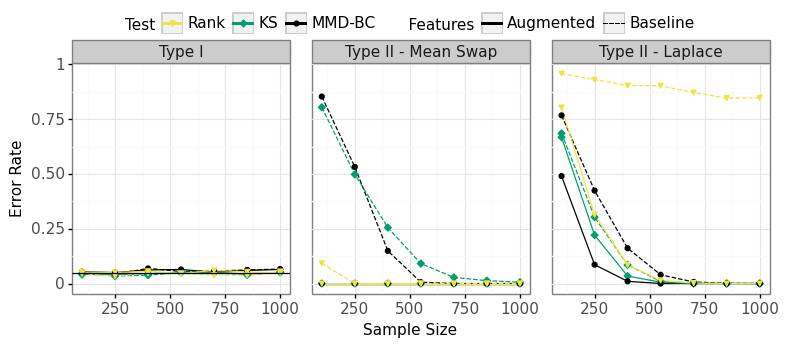
\includegraphics[width=\textwidth]{figures/results_1.png}
    \caption{
        Experiment 1 type-I/II error rates of BC tests with varying test functions, calculated over 1000 trials. 
        For the BC simulator, we set $L=500$.
        For the benchmark Rank test, we set $\tilde{L}=5$.
    }
    \label{fig:ex1_aux}
\end{figure}

When $\sigma_{\epsilon} \ll \sigma$, the sample autocorrelation in the successive conditional sampler is very high, and successive-conditional tests require many more samples than backwards-conditional tests to push their type-I error rates below $\alpha=0.05$. Tuning $\sigma_{\epsilon}$ thus enables analysis of test behavior given samplers with varying mixing speeds (see Appendix). As we might expect, when the sample autocorrelation is very high, the MMD-SC and Geweke tests always reject the null hypothesis. As $\sigma_{\epsilon}$ increases and the autocorrelation falls, their type-I error rates fall. Type-II error rates improve across all tests with mixing speed.

\subsection{Reversible-jump Bayesian Lasso}
\label{section:ex2}
This example is similar to \cite{chen_bayesian_2011}, but replaces improper priors with proper ones. Given a fixed design matrix $X$ and observed outcomes $y$, we wish to learn the distribution of the parameters $\beta$ and $\sigma$ under the sparse linear model
\begin{equation}
    y = X\beta + \mathbf{\epsilon}, \quad \mathbf{\epsilon} \sim \mathcal{N}(\mathbf{0}, \sigma^{2} \mathbf{I})
    \label{eq:ex2}
\end{equation}
We place a truncated Poisson prior $p(\ell|\lambda)$ on the number of nonzero coefficients $\beta_{j}$ and an inverse-gamma prior on $\sigma^{2}$. Because the number of nonzero coefficients $\beta_{j}$ in \eqref{eq:ex2} is unknown, the algorithm must draw from parameter spaces of varying dimension. We implement a reversible-jump step \citep{green_reversible_1995} based on \cite{chen_bayesian_2011} that achieves this; see the Appendix for full details. We fix $X \in \mathbb{R}^{3 \times 3}$, with $\lambda=1$ and hyperparameters $\tau=1, a=3, b=1$. The reversible jump random walk sizes are set to $\epsilon_\text{update}= \epsilon_\text{birth}=1$.

Each iteration of the reversible-jump MCMC posterior sampler takes two steps in random order. A Gibbs step updates $\sigma^{2}$, which is straightforward due to the conjugacy of the Inverse Gamma prior on $\sigma^{2}$. A reversible jump step that traverses parameter spaces with varying $\ell$. We accept the birth-death proposal $\theta'$ with probability 
\begin{equation}
    A(\theta'|\theta) = \min{\left(\frac{p(y, \theta' | X )}{p(y, \theta | X )} \frac{p(\theta' \rightarrow \theta)}{p(\theta \rightarrow \theta')}, 1\right)} \\
\end{equation}

We introduce several errors into the the posterior sampler summarized in Table \ref{tab:ex2_errors}. The first error affects the Metropolis-Hastings acceptance probabilities used in the birth/death moves; it omits the jump probabilities $p(\theta' \rightarrow \theta), p(\theta \rightarrow \theta')$ from the calculation. The second error affects all of the Metropolis-Hastings acceptance probabilities. The truncated Poisson factors $p(\ell|\lambda)$  of the joint probabilities have incorrect denominator $(\ell-1)!$ rather than $\ell!$. 
For the MMD tests, we use the same kernel as in the previous experiment;  $k_{\mathrm{IMQ}}(g, \tilde{g}) + k_{\mathrm{IMQ}}(h, \tilde{h})$. The benchmark tests use all first and second moments of $\{\beta,\sigma\}$ and the evaluations of the likelihood and prior.
The results are shown in Figure \ref{fig:ex2_comparison}.

The autocorrelation in the successive-conditional samples results in elevated rejection rates for the Geweke test. Despite using the same samples, the MMD-SC test better controls type-I error rates. Its type-II error rates are decidedly worse than the other tests, however. Due to the independence of their samples, the other backwards-conditional tests are most efficient.

\begin{table}
    \caption{Experiment 2 intentional errors in posterior sampler}
    \label{tab:ex2_errors}
    \centering
    \begin{tabular}{l|l|l|l}
    \toprule
          Error & Components & Incorrect & Correct \\
    \midrule  
         Transition & $A_{\text{birth}}(\theta'|\theta)$, $A_{\text{death}}(\theta'|\theta)$  &  $\ldots\frac{P(y, \theta' | X )}{P(y, \theta | X )}\ldots$ & $\ldots\frac{P(y, \theta' | X )}{P(y, \theta | X )} \frac{P(\theta' \rightarrow \theta)}{P(\theta \rightarrow \theta')}\ldots$\\
         Poisson & $P(y, \theta' | X )$, $P(y, \theta | X )$ & $\ldots \frac{\exp{(-\lambda)} \lambda^{\ell}}{(\ell-1)!} \ldots$ & $\ldots \frac{\exp{(-\lambda)} \lambda^{\ell}}{\ell!} \ldots$ \\
    \bottomrule
    \end{tabular}
\end{table}

\begin{figure}[H]
    \centering
    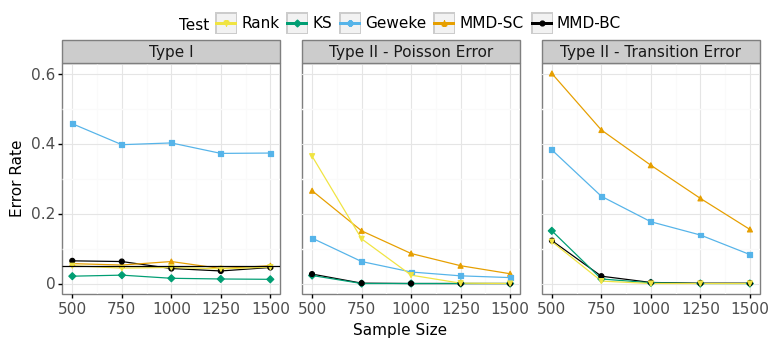
\includegraphics[width=\textwidth]{figures/results_2.png}
    \caption{Experiment 2 type-I/II error rates calculated over 1000 trials with $\alpha=0.05$.
    We set $j=5$ for the SC simulator, and $L=500$ for both the SC and BC simulators. For the benchmark Rank test, we set $\tilde{L}=5$. The Geweke window size was set to $8\%$ of the sample size.
    }
    \label{fig:ex2_comparison}
\end{figure}

\subsection{Metropolis-Hastings for Learning DAG Structure}
The purpose of this experiment is to show that the MMD tests can be easily generalized to spaces other than $\mathbb{R}^{d}$ on which we can define a kernel. We are interested in inferring the structure $\mathcal{G}$ of a directed acyclic graph (DAG) given observed data. $\mathcal{G}=(V,E)$ is a set of vertices (nodes) and edges encoding conditional independence relationships between nodes. In particular, the value of a child node $y_{j}$ depends only on the value of its parent nodes. A node with no parents is called a root, and a node with no children is called a leaf. A graph structure may thus be represented by an adjacency matrix; entry $(i,j)=1$ indicates that $y_{i}$ is the parent of child node $y_{j}$; $(i,j)=0$ otherwise. In an acyclic graph structure, a node cannot be a descendant of itself.

Let $\mathbf{pa}(y_{j})$ denote the set of parent nodes of node $y_{j}$. In this experiment, we place a uniform  prior on the structure; $\pi(\mathcal{G}) \propto 1$. Given structure $\mathcal{G}$ and data $y$, we draw each root node $y_{r} \sim \mathcal{N}(0, \epsilon^2)$ and each child node $y_{j}|\mathbf{pa}(y_{j}) \sim \mathcal{N}(\sum_{z \in \mathbf{pa}(y_{j})} z, \epsilon^2)$. The likelihood is thus
\begin{equation}
    p(y|\mathcal{G}) = \prod_{j=1}^{n}  p(y_{j}|\mathcal{G}) = \prod_{j=1}^{n} p(y_{j}|\mathbf{pa}(y_{j}))
\end{equation}

The sampling algorithm we consider is detailed in section 2 of \cite{grzegorczyk_improving_2008}. 
Given a graph structure $\mathcal{G}$, the proposal structure $\mathcal{G}'$ is sampled uniformly from the neighborhood $\mathbf{Ne}(\mathcal{G})$, the union of $\mathcal{G}$ and the set of all DAGs that can be reached by adding, deleting, or reversing an edge. We use the method of \cite{kuipers_uniform_2015} to sample DAGs uniformly.

The sampler errors considered all affect the Metropolis-Hastings acceptance probability.
\begin{equation}
A(\mathcal{G}'|\mathcal{G}) = \min{\left(\frac{p(y|\mathcal{G}')|\mathbf{Ne}(\mathcal{G})|}{p(y|\mathcal{G})|\mathbf{Ne}(\mathcal{G}')|}, 1\right)}
\end{equation}
Specifically, they alter the calculation of $|\mathbf{Ne}(\mathcal{G})|$. In the first error, we count all \textit{graphs} that can be reached by modifying a single edge, regardless of whether the modification induces a cycle. In the subtler second error, we double-count the DAGs that can be reached by reversing an edge. These errors are summarized in Table \ref{tab:ex3_errors}.

We examine two sets of tests: one on $\mathbb{R}^{d}$ and the other on the space of DAGs. For the former, we treat each entry in the adjacency matrix representation of the sampled graph structure $\mathcal{G}$ as a binary parameter. Since the parameters are discrete, we cannot apply the KS or Rank tests as benchmarks. For the Geweke test, we use a subset of the the first and second moments of these parameters as test functions; all moments that must be zero for the graph to be cyclic are excluded. We include the evaluation of the likelihood $p(y|\mathcal{G})$ and omit the evaluation of the uniform prior $\pi(\mathcal{G})$ as it is constant. The MMD test functions use the IMQ sum kernel from previous experiments.

Using the adjacency matrix representation, the number of test functions scales poorly with graph size; for example, just the first moments are $\mathcal{O}(n^2)$, and including the second moments is $\mathcal{O}(n^4)$. Thus, the Geweke test will lose power from conducting and correcting for so many tests. The rapidly scaling dimensionality of the problem also will pose problems for the MMD tests. However, unlike the Geweke test, the MMD tests can be adapted to these settings using kernels on graphs; we chose random walk kernels \citep{gartner_graph_2003, vishwanathan_fast_2006}. As a final benchmark in DAG space, we also include a $\chi^{2}$ test of backwards-conditional sample DAG frequencies; this is an idealized test since it uses true expected frequencies. The results are shown in Figure \ref{fig:ex3_comparison}. 

As we might expect, the $\chi^{2}$ test performs best. The Geweke test lags far behind, but does reasonably well; the test functions are enough capture the errors. The MMD tests using the adjacency matrix features perform worst; the problem is too high-dimensional in $\mathbb{R}^{d}$ for the tests to be very efficient. In contrast, using the random walk kernel, the MMD tests are able outperform the Geweke test in detecting the Cyclic Check error, almost matching the $\chi^{2}$ test; however, the Rev Count type-II error degrades. In fact, random walk kernels cannot distinguish between isomorphic graphs.

To the extent that we wish to perform tests directly on the DAG space, the $\chi^{2}$ test is strictly superior to the graph kernel MMD tests; it is consistent and much faster. On the other hand, testing only on the DAG space also will miss discrepancies in the relationship between $\mathcal{G}$ and $y$. Trivially, if our posterior sampler used a uniform proposal distribution but wrongly set the acceptance probability to unity, none of these tests would pick up on the error, which would instead influence the likelihood feature. A preferable way to check the structure sampler would thus be to run the $\chi^{2}$ test on the sampled structures along with the KS test on the auxiliary features.

Here, the DAG space is discrete and thus the $\chi^{2}$ test is a better choice, but the MMD tests may also be applied to MCMC schemes on continuous domains such as random matrices \citep{beskos_mcmc_2021} or functions \citep{jeltsch_mcmc_2009}, given the right kernel. \ajsay{todo: cite examples of kernels on random matrices / functions...} 
The primary concern outside of $\mathbb{R}^{d}$ is that, if we do not have access to characteristic kernels, the consistency of the MMD tests is consequently not guaranteed. However, the tests may still protect against some mistakes.

\begin{table}
    \caption{Experiment 3 intentional errors in posterior sampler}
    \label{tab:ex3_errors}
    \centering
    \begin{tabular}{l|l|l|l}
    \toprule
          Error & Components & Incorrect & Correct \\
    \midrule  
         Cyclic Check & $|\mathbf{Ne}(\mathcal{G})|, |\mathbf{Ne}(\mathcal{G}')|$ & Count graph neighbors & Count DAG neighbors \\
         Rev Count & $|\mathbf{Ne}(\mathcal{G})|, |\mathbf{Ne}(\mathcal{G}')|$ & Count reversals twice & Count reversals once \\
    \bottomrule
    \end{tabular}
\end{table}


\begin{figure}
    \centering
    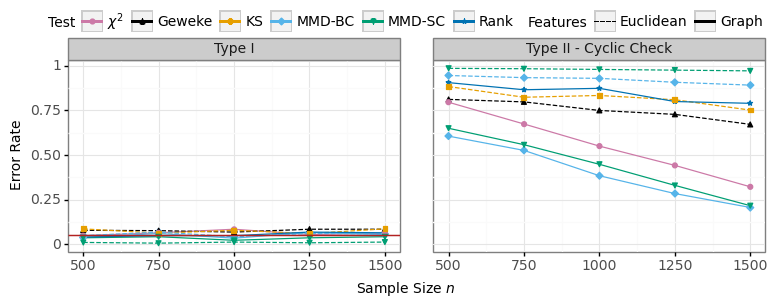
\includegraphics[width=\textwidth]{figures/results_3.png}
    \caption{Experiment 3 type-I/II error rates calculated over 300 trials with $\alpha=0.05$. We set $j=5$ for the SC simulator, and $L=500$ for both the SC and BC simulators. The Geweke window size was set to $8\%$ of the sample size.
    }
    % For the Geweke test, we use a subset of the the first and second moments of these parameters as test functions; all moments that must be zero for the graph to be cyclic are excluded.
    \label{fig:ex3_comparison}
\end{figure}


\section{Broader Impact}
MCMC algorithms are commonly used across the natural and social sciences. However, they can be quite complex and error-prone. Compared to previous methods, our MCMC tests come with improved theoretical guarantees based on kernels and thus are of practical use to both researchers and practitioners. They may improve the quality of related academic literature by preventing the propagation of erroneous inferences, as well as easing correction of hitherto undetected mistakes.

% \subsection{Style}

% Papers to be submitted to NeurIPS 2021 must be prepared according to the
% instructions presented here. Papers may only be up to {\bf nine} pages long,
% including figures. Additional pages \emph{containing only acknowledgments and
% references} are allowed. Papers that exceed the page limit will not be
% reviewed, or in any other way considered for presentation at the conference.

% The margins in 2021 are the same as those in 2007, which allow for $\sim$$15\%$
% more words in the paper compared to earlier years.

% Authors are required to use the NeurIPS \LaTeX{} style files obtainable at the
% NeurIPS website as indicated below. Please make sure you use the current files
% and not previous versions. Tweaking the style files may be grounds for
% rejection.

% \subsection{Retrieval of style files}

% The style files for NeurIPS and other conference information are available on
% the World Wide Web at
% \begin{center}
%   \url{http://www.neurips.cc/}
% \end{center}
% The file \verb+neurips_2021.pdf+ contains these instructions and illustrates the
% various formatting requirements your NeurIPS paper must satisfy.

% The only supported style file for NeurIPS 2021 is \verb+neurips_2021.sty+,
% rewritten for \LaTeXe{}.  \textbf{Previous style files for \LaTeX{} 2.09,
%   Microsoft Word, and RTF are no longer supported!}

% The \LaTeX{} style file contains three optional arguments: \verb+final+, which
% creates a camera-ready copy, \verb+preprint+, which creates a preprint for
% submission to, e.g., arXiv, and \verb+nonatbib+, which will not load the
% \verb+natbib+ package for you in case of package clash.

% \paragraph{Preprint option}
% If you wish to post a preprint of your work online, e.g., on arXiv, using the
% NeurIPS style, please use the \verb+preprint+ option. This will create a
% nonanonymized version of your work with the text ``Preprint. Work in progress.''
% in the footer. This version may be distributed as you see fit. Please \textbf{do
%   not} use the \verb+final+ option, which should \textbf{only} be used for
% papers accepted to NeurIPS.

% At submission time, please omit the \verb+final+ and \verb+preprint+
% options. This will anonymize your submission and add line numbers to aid
% review. Please do \emph{not} refer to these line numbers in your paper as they
% will be removed during generation of camera-ready copies.

% The file \verb+neurips_2021.tex+ may be used as a ``shell'' for writing your
% paper. All you have to do is replace the author, title, abstract, and text of
% the paper with your own.

% The formatting instructions contained in these style files are summarized in
% Sections \ref{gen_inst}, \ref{headings}, and \ref{others} below.

% \section{General formatting instructions}
% \label{gen_inst}

% The text must be confined within a rectangle 5.5~inches (33~picas) wide and
% 9~inches (54~picas) long. The left margin is 1.5~inch (9~picas).  Use 10~point
% type with a vertical spacing (leading) of 11~points.  Times New Roman is the
% preferred typeface throughout, and will be selected for you by default.
% Paragraphs are separated by \nicefrac{1}{2}~line space (5.5 points), with no
% indentation.

% The paper title should be 17~point, initial caps/lower case, bold, centered
% between two horizontal rules. The top rule should be 4~points thick and the
% bottom rule should be 1~point thick. Allow \nicefrac{1}{4}~inch space above and
% below the title to rules. All pages should start at 1~inch (6~picas) from the
% top of the page.

% For the final version, authors' names are set in boldface, and each name is
% centered above the corresponding address. The lead author's name is to be listed
% first (left-most), and the co-authors' names (if different address) are set to
% follow. If there is only one co-author, list both author and co-author side by
% side.

% Please pay special attention to the instructions in Section \ref{others}
% regarding figures, tables, acknowledgments, and references.

% \section{Headings: first level}
% \label{headings}

% All headings should be lower case (except for first word and proper nouns),
% flush left, and bold.

% First-level headings should be in 12-point type.

% \subsection{Headings: second level}

% Second-level headings should be in 10-point type.

% \subsubsection{Headings: third level}

% Third-level headings should be in 10-point type.

% \paragraph{Paragraphs}

% There is also a \verb+\paragraph+ command available, which sets the heading in
% bold, flush left, and inline with the text, with the heading followed by 1\,em
% of space.

% \section{Citations, figures, tables, references}
% \label{others}

% These instructions apply to everyone.

% \subsection{Citations within the text}

% The \verb+natbib+ package will be loaded for you by default.  Citations may be
% author/year or numeric, as long as you maintain internal consistency.  As to the
% format of the references themselves, any style is acceptable as long as it is
% used consistently.

% The documentation for \verb+natbib+ may be found at
% \begin{center}
%   \url{http://mirrors.ctan.org/macros/latex/contrib/natbib/natnotes.pdf}
% \end{center}
% Of note is the command \verb+\citet+, which produces citations appropriate for
% use in inline text.  For example,
% \begin{verbatim}
%   \citet{hasselmo} investigated\dots
% \end{verbatim}
% produces
% \begin{quote}
%   Hasselmo, et al.\ (1995) investigated\dots
% \end{quote}

% If you wish to load the \verb+natbib+ package with options, you may add the
% following before loading the \verb+neurips_2021+ package:
% \begin{verbatim}
% \PassOptionsToPackage{options}{natbib}
% \end{verbatim}

% If \verb+natbib+ clashes with another package you load, you can add the optional
% argument \verb+nonatbib+ when loading the style file:
% \begin{verbatim}
%   \usepackage[nonatbib]{neurips_2021}
% \end{verbatim}

% As submission is double blind, refer to your own published work in the third
% person. That is, use ``In the previous work of Jones et al.\ [4],'' not ``In our
% previous work [4].'' If you cite your other papers that are not widely available
% (e.g., a journal paper under review), use anonymous author names in the
% citation, e.g., an author of the form ``A.\ Anonymous.''

% \subsection{Footnotes}

% Footnotes should be used sparingly.  If you do require a footnote, indicate
% footnotes with a number\footnote{Sample of the first footnote.} in the
% text. Place the footnotes at the bottom of the page on which they appear.
% Precede the footnote with a horizontal rule of 2~inches (12~picas).

% Note that footnotes are properly typeset \emph{after} punctuation
% marks.\footnote{As in this example.}

% \subsection{Figures}

% \begin{figure}
%   \centering
%   \fbox{\rule[-.5cm]{0cm}{4cm} \rule[-.5cm]{4cm}{0cm}}
%   \caption{Sample figure caption.}
% \end{figure}

% All artwork must be neat, clean, and legible. Lines should be dark enough for
% purposes of reproduction. The figure number and caption always appear after the
% figure. Place one line space before the figure caption and one line space after
% the figure. The figure caption should be lower case (except for first word and
% proper nouns); figures are numbered consecutively.

% You may use color figures.  However, it is best for the figure captions and the
% paper body to be legible if the paper is printed in either black/white or in
% color.

% \subsection{Tables}

% All tables must be centered, neat, clean and legible.  The table number and
% title always appear before the table.  See Table~\ref{sample-table}.

% Place one line space before the table title, one line space after the
% table title, and one line space after the table. The table title must
% be lower case (except for first word and proper nouns); tables are
% numbered consecutively.

% Note that publication-quality tables \emph{do not contain vertical rules.} We
% strongly suggest the use of the \verb+booktabs+ package, which allows for
% typesetting high-quality, professional tables:
% \begin{center}
%   \url{https://www.ctan.org/pkg/booktabs}
% \end{center}
% This package was used to typeset Table~\ref{sample-table}.

% \begin{table}
%   \caption{Sample table title}
%   \label{sample-table}
%   \centering
%   \begin{tabular}{lll}
%     \toprule
%     \multicolumn{2}{c}{Part}                   \\
%     \cmidrule(r){1-2}
%     Name     & Description     & Size ($\mu$m) \\
%     \midrule
%     Dendrite & Input terminal  & $\sim$100     \\
%     Axon     & Output terminal & $\sim$10      \\
%     Soma     & Cell body       & up to $10^6$  \\
%     \bottomrule
%   \end{tabular}
% \end{table}

% \section{Final instructions}

% Do not change any aspects of the formatting parameters in the style files.  In
% particular, do not modify the width or length of the rectangle the text should
% fit into, and do not change font sizes (except perhaps in the
% \textbf{References} section; see below). Please note that pages should be
% numbered.

% \section{Preparing PDF files}

% Please prepare submission files with paper size ``US Letter,'' and not, for
% example, ``A4.''

% Fonts were the main cause of problems in the past years. Your PDF file must only
% contain Type 1 or Embedded TrueType fonts. Here are a few instructions to
% achieve this.

% \begin{itemize}

% \item You should directly generate PDF files using \verb+pdflatex+.

% \item You can check which fonts a PDF files uses.  In Acrobat Reader, select the
%   menu Files$>$Document Properties$>$Fonts and select Show All Fonts. You can
%   also use the program \verb+pdffonts+ which comes with \verb+xpdf+ and is
%   available out-of-the-box on most Linux machines.

% \item The IEEE has recommendations for generating PDF files whose fonts are also
%   acceptable for NeurIPS. Please see
%   \url{http://www.emfield.org/icuwb2010/downloads/IEEE-PDF-SpecV32.pdf}

% \item \verb+xfig+ "patterned" shapes are implemented with bitmap fonts.  Use
%   "solid" shapes instead.

% \item The \verb+\bbold+ package almost always uses bitmap fonts.  You should use
%   the equivalent AMS Fonts:
% \begin{verbatim}
%   \usepackage{amsfonts}
% \end{verbatim}
% followed by, e.g., \verb+\mathbb{R}+, \verb+\mathbb{N}+, or \verb+\mathbb{C}+
% for $\mathbb{R}$, $\mathbb{N}$ or $\mathbb{C}$.  You can also use the following
% workaround for reals, natural and complex:
% \begin{verbatim}
%   \newcommand{\RR}{I\!\!R} %real numbers
%   \newcommand{\Nat}{I\!\!N} %natural numbers
%   \newcommand{\CC}{I\!\!\!\!C} %complex numbers
% \end{verbatim}
% Note that \verb+amsfonts+ is automatically loaded by the \verb+amssymb+ package.

% \end{itemize}

% If your file contains type 3 fonts or non embedded TrueType fonts, we will ask
% you to fix it.

% \subsection{Margins in \LaTeX{}}

% Most of the margin problems come from figures positioned by hand using
% \verb+\special+ or other commands. We suggest using the command
% \verb+\includegraphics+ from the \verb+graphicx+ package. Always specify the
% figure width as a multiple of the line width as in the example below:
% \begin{verbatim}
%   \usepackage[pdftex]{graphicx} ...
%   \includegraphics[width=0.8\linewidth]{myfile.pdf}
% \end{verbatim}
% See Section 4.4 in the graphics bundle documentation
% (\url{http://mirrors.ctan.org/macros/latex/required/graphics/grfguide.pdf})

% A number of width problems arise when \LaTeX{} cannot properly hyphenate a
% line. Please give LaTeX hyphenation hints using the \verb+\-+ command when
% necessary.

\begin{ack}
Use unnumbered first level headings for the acknowledgments. All acknowledgments
go at the end of the paper before the list of references. Moreover, you are required to declare
funding (financial activities supporting the submitted work) and competing interests (related financial activities outside the submitted work).
More information about this disclosure can be found at: \url{https://neurips.cc/Conferences/2021/PaperInformation/FundingDisclosure}.

Do {\bf not} include this section in the anonymized submission, only in the final paper. You can use the \texttt{ack} environment provided in the style file to autmoatically hide this section in the anonymized submission.
\end{ack}

% \section*{References}
\small{
\bibliography{references}
% [1] Alexander, J.A.\ \& Mozer, M.C.\ (1995) Template-based algorithms for
% connectionist rule extraction. In G.\ Tesauro, D.S.\ Touretzky and T.K.\ Leen
% (eds.), {\it Advances in Neural Information Processing Systems 7},
% pp.\ 609--616. Cambridge, MA: MIT Press.

% [2] Bower, J.M.\ \& Beeman, D.\ (1995) {\it The Book of GENESIS: Exploring
%   Realistic Neural Models with the GEneral NEural SImulation System.}  New York:
% TELOS/Springer--Verlag.

% [3] Hasselmo, M.E., Schnell, E.\ \& Barkai, E.\ (1995) Dynamics of learning and
% recall at excitatory recurrent synapses and cholinergic modulation in rat
% hippocampal region CA3. {\it Journal of Neuroscience} {\bf 15}(7):5249-5262.
}

%%%%%%%%%%%%%%%%%%%%%%%%%%%%%%%%%%%%%%%%%%%%%%%%%%%%%%%%%%%%
\section*{Checklist}

%%% BEGIN INSTRUCTIONS %%%
The checklist follows the references.  Please
read the checklist guidelines carefully for information on how to answer these
questions.  For each question, change the default \answerTODO{} to \answerYes{},
\answerNo{}, or \answerNA{}.  You are strongly encouraged to include a {\bf
justification to your answer}, either by referencing the appropriate section of
your paper or providing a brief inline description.  For example:
\begin{itemize}
  \item Did you include the license to the code and datasets? \answerYes{See Section~\ref{gen_inst}.}
  \item Did you include the license to the code and datasets? \answerNo{The code and the data are proprietary.}
  \item Did you include the license to the code and datasets? \answerNA{}
\end{itemize}
Please do not modify the questions and only use the provided macros for your
answers.  Note that the Checklist section does not count towards the page
limit.  In your paper, please delete this instructions block and only keep the
Checklist section heading above along with the questions/answers below.
%%% END INSTRUCTIONS %%%

\begin{enumerate}

\item For all authors...
\begin{enumerate}
  \item Do the main claims made in the abstract and introduction accurately reflect the paper's contributions and scope?
    \answerTODO{}
  \item Did you describe the limitations of your work?
    \answerTODO{}
  \item Did you discuss any potential negative societal impacts of your work?
    \answerTODO{}
  \item Have you read the ethics review guidelines and ensured that your paper conforms to them?
    \answerTODO{}
\end{enumerate}

\item If you ran experiments...
\begin{enumerate}
  \item Did you include the code, data, and instructions needed to reproduce the main experimental results (either in the supplemental material or as a URL)?
    \answerTODO{}
  \item Did you specify all the training details (e.g., data splits, hyperparameters, how they were chosen)?
    \answerTODO{}
	\item Did you report error bars (e.g., with respect to the random seed after running experiments multiple times)?
    \answerTODO{}
	\item Did you include the total amount of compute and the type of resources used (e.g., type of GPUs, internal cluster, or cloud provider)?
    \answerTODO{}
\end{enumerate}

\item If you are using existing assets (e.g., code, data, models) or curating/releasing new assets...
\begin{enumerate}
  \item If your work uses existing assets, did you cite the creators?
    \answerTODO{}
  \item Did you mention the license of the assets?
    \answerTODO{}
  \item Did you include any new assets either in the supplemental material or as a URL?
    \answerTODO{}
  \item Did you discuss whether and how consent was obtained from people whose data you're using/curating?
    \answerTODO{}
  \item Did you discuss whether the data you are using/curating contains personally identifiable information or offensive content?
    \answerTODO{}
\end{enumerate}

\end{enumerate}

%%%%%%%%%%%%%%%%%%%%%%%%%%%%%%%%%%%%%%%%%%%%%%%%%%%%%%%%%%%%

\appendix

\section{Baseline methods}
\subsection{Geweke test}
The Geweke test \citep{geweke_getting_2004} compares (estimates of) the expectations of hand-picked features (\emph{test functions}) under both the forward and backward joints. 
Specifically, let $g: \mathcal{Y}\times \Theta\to \mathbb{R}$ denote a test function, and let  $S_f=\{(y_i, \theta_i)\}_{i=1}^n$ be samples from the forward joint and $S_b=\{(\tilde{y}_i, \tilde{\theta}_i)\}_{i=1}^n$ be ones from the backward joint.
Then, the z-score 
% $\sqrt{n}(\hat{\bar{g}} - \hat{\tilde{g}})/\sqrt{\hat{\sigma^{2}}+\hat{\tilde{\sigma}}^{2}}$
\begin{equation}
    \frac{\bar{g}(S_f) - \bar{g}(S_b)}{\sqrt{ \frac{\hat{\sigma}^{2}}{N} + \frac{\hat{\tilde{\sigma}}^{2}}{N}}} 
    % \xrightarrow[]{d} \mathcal{N}(0, 1)
    \label{eq:geweke}
\end{equation}
asymptotically follows the standard Gaussian if $\tilde{\pi}(\theta\given y)=\pi(\theta\given y)$, where $\bar{g}(S) = \frac{1}{n}\sum_{(y,\theta) \in S}g(y, \theta)$ and $\hat{\sigma}, \hat{\tilde{\sigma}}$ are estimated variances. 
The width of the window estimator $\hat{\tilde{\sigma}}$ can be set to account for the serial dependence in the backward joint samples.
\subsection{\cite{talts_validating_2018}}
% \cite{talts_validating_2018} take a similar approach under the assumption that the posterior is absolutely continuous.
The authors draw samples using the BC algorithm, then compute univariate rank statistics of a draw from the prior among the thinned, approximately independent posterior samples; if there is no error, the rank statistics should be discretely uniformly distributed. 
The authors suggest examining histograms of the rank statistics to better understand errors rather than conducting a formal test.

\subsection{Rank statistic approach of \cite{gandy_unit_2020}}
% Rather than conducting a (battery of) two-sample tests, we may take a parametric approach.
The rank test from \cite{gandy_unit_2020} requires reversibility of the MCMC sampler. It draws a sample $\theta_{l}$ from the prior, with the associated index $l$ drawn uniformly from $\{1,\ldots,\tilde{L}\}$. The sampler is then run forward and backward to generate samples $\theta_{1}, \ldots, \theta_{l-1}$ and $\theta_{l+1}, \ldots, \theta_{\tilde{L}} $. Under the null, the rank statistic of $\theta_{l}$ among the other samples should be uniformly distributed; after many repeated simulations, this is verified using a $\chi^{2}$ test.



\section{Experiment details}
\subsection{Experiment 1}
\subsubsection{Effect of sampler mixing speed}
\begin{figure}[H]
    \centering
    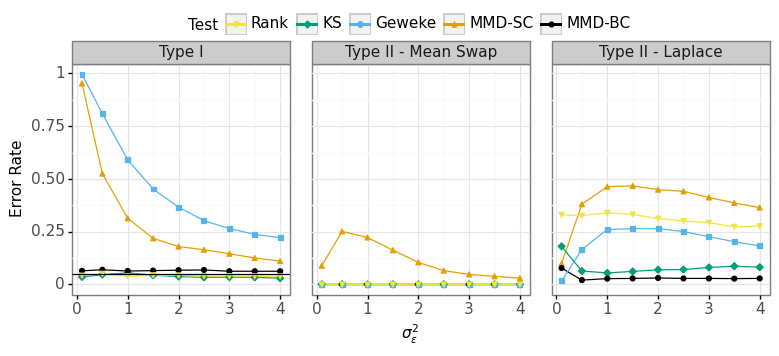
\includegraphics[width=\textwidth]{figures/results_1a.png}
    \caption{Experiment 1 type-I/II error rates against $\sigma_{\epsilon}$, calculated over 1000 trials with a sample size of 250. As $\sigma_{\epsilon}$ increases, autocorrelation in the Gibbs sampler decreases and mixing speed increases. We set $j=5$ for the SC simulator, and $L=500$ for both the SC and BC simulators. For the benchmark Rank test, we set $\tilde{L}=5$.}
    \label{fig:ex1_auto}
\end{figure}

\subsubsection{Effect of varying BC simulator burn-in}
\begin{figure}[H]
    \centering
    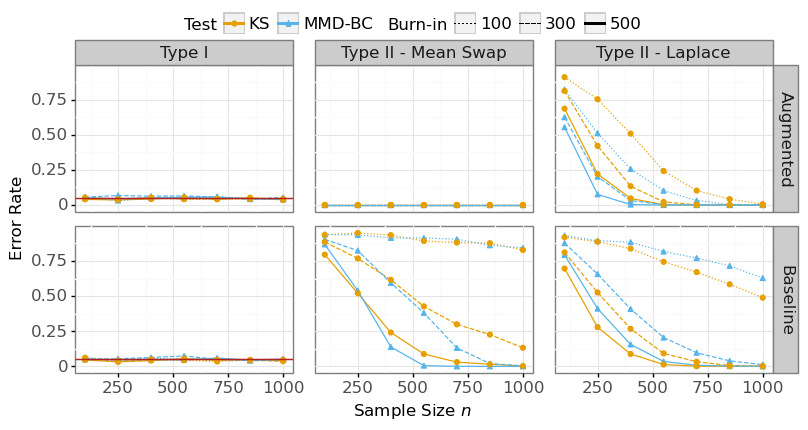
\includegraphics[width=\textwidth]{figures/results_1b.png}
    \caption{Experiment 1 type-I/II error rates calculated over 1000 trials. The top panels uses the likelihood- and prior-augmented test functions and the bottom panels use the baseline as discussed in the text. We set $\sigma_{\epsilon}^{2}=0.1$.}
    \label{fig:ex1_auto}
\end{figure}

\subsection{Experiment 2: Reversible Jump Sampler Implementation}
\label{appendix:ex2}
The prior is defined by
\begin{equation}
  \pi(\theta|\tau, a, b ) = p(\ell|\lambda) p(\mathbf{\gamma}|\ell) p(\beta_{j} | \tau, \gamma) p(\sigma^{2} | a, b)
\end{equation}
where
\begin{equation}
  p(\ell|\lambda) = \frac{\exp{(-\lambda)} \lambda^{\ell}}{C\ell!}, \quad \ell \in \{1,\ldots, p\}
\end{equation}
\begin{equation}
  p(\mathbf{\gamma}|\ell) = {p\choose \ell}^{-1}
\end{equation}
\begin{equation}
  p(\beta_{j} | \tau, \gamma ) = \begin{cases} (2\tau)^{-1}\exp(-\frac{|\beta_{j}|}{\tau}) & j \in \mathbf{\gamma} \\ \delta(\beta_{j}) & \text{otherwise} \end{cases}
\end{equation}
\begin{equation}
    p(\sigma^{2} | a, b) = \frac{b^{a}}{\Gamma(a)} (\sigma^{2})^{-a-1} \exp{\left(-\frac{b}{\sigma^{2}}\right)}
\end{equation}
$C$ is a normalization constant, $\delta$ is the Dirac delta function, and $\mathbf{\gamma}$ is a vector of the nonzero indices of $\beta$.
The likelihood is given by
\begin{equation}
  p(y | \sigma, \beta, X ) = (2\pi)^{-\frac{n}{2}} \sigma^{-n} \exp{\left(-\frac{\Vert y-X\beta\Vert^{2}_{2}}{2\sigma^{2}}\right)}
\end{equation}
The joint probability is then
\begin{equation}
    \begin{aligned}
         p(y, \theta | X ) \propto &\sigma^{-n} \exp{\left(-\frac{\Vert  y-X\beta\Vert^{2}_{2}}{2\sigma^{2}}\right)} \times \\ 
         & \frac{\exp{(-\lambda)} \lambda^{\ell}}{\ell!} {p\choose \ell}^{-1} \prod_{j\in \mathbf{\gamma}} (2\tau)^{-1}\exp\left(-\frac{|\beta_{j}|}{\tau}\right) \prod_{j' \notin \mathbf{\gamma}} \delta(\beta_{j'}) \frac{b^{a}}{\Gamma(a)} (\sigma^{2})^{-a-1} \exp{\left(-\frac{b}{\sigma^{2}}\right)}
    \end{aligned}
    \label{eq:ex2_joint}
\end{equation}

Each iteration of the reversible-jump MCMC posterior sampler takes two steps in random order. The first is a Gibbs step. By conjugacy,
\begin{equation}
    \sigma^{2} | y, X, \beta \sim \mathcal{IG}\left(a + \frac{n}{2}, b + \frac{\sum_{i=1}^{n}(y_{i}-x_{i}\beta)^{2} }{2}\right)
\end{equation}
where $x_{i}$ denotes row $i$ of $X$.

The second is a reversible jump step. We start by proposing $\ell' \in \{\ell-1, \ell, \ell+1\}$ uniformly at random, disallowing $\ell<1$ and $\ell>p$. Thus, when $\ell \in \{1,p\}$, there are only two valid proposals, not three. Then, depending on the $\ell'$ proposed, we complete the proposal $\theta'$ via one of the following
\begin{itemize}
    \item Update: $\ell' = \ell$
    \begin{enumerate}
        \item Choose $j \in \{1, \ldots, \ell\}$ uniformly at random
        \item Propose $\mathbf{\gamma}' = \mathbf{\gamma}, \beta'_{j} = \beta_{j} + \mathcal{N}(0, \epsilon_{\text{update}}), \beta'_{i \neq j} = \beta_{i}$
        \item $P(\theta' \rightarrow \theta) = P(\theta \rightarrow \theta')=\mathcal{N}(\beta_{j}'; \beta_{j},\epsilon_{\text{update}})=\mathcal{N}(\beta_{j}; \beta_{j}',\epsilon_{\text{update}})$
    \end{enumerate}
\end{itemize}

\begin{itemize}
    \item Birth: $\ell' = \ell+1$
    \begin{enumerate}
        \item Choose $j \in \{\ell+1, \ldots, p\}$ uniformly at random
        \item Propose $\mathbf{\gamma}' = \mathbf{\gamma} \cup j$
        \item Propose $\beta'_{j} = \mathcal{N}(0, \epsilon_{\text{birth}}), \beta'_{i \neq j} = \beta_{i}$
        \item $p(\theta' \rightarrow \theta) = \begin{cases}\frac{1}{2}\frac{1}{\ell'} & \ell'=p \\ \frac{1}{3} \frac{1}{\ell'} & 1<\ell<p \end{cases} $
        \item $p(\theta \rightarrow \theta') = \begin{cases}\frac{1}{2}\frac{1}{p-\ell} \mathcal{N}(\beta_{j}'; 0,\epsilon_{\text{birth}}) & \ell=1 \\ \frac{1}{3} \frac{1}{p-\ell} \mathcal{N}(\beta_{j}'; 0,\epsilon_{\text{birth}}) & 1<\ell<p \end{cases} $
    \end{enumerate}
\end{itemize}

\begin{itemize}
    \item Death: $\ell' = \ell-1$
    \begin{enumerate}
        \item Choose $j \in \{1, \ldots, \ell\}$ uniformly at random
        \item Propose $\mathbf{\gamma}' = \mathbf{\gamma} \setminus j$ 
        \item Propose $\beta'_{j} = 0, \beta'_{i \neq j} = \beta_{i}$
        \item $p(\theta' \rightarrow \theta) = \begin{cases}\frac{1}{2}\frac{1}{p-\ell'} \mathcal{N}(\beta_{j}; 0,\epsilon_{\text{birth}}) & k'=1 \\ \frac{1}{3} \frac{1}{p-\ell'} \mathcal{N}(\beta_{j}; 0,\epsilon_{\text{birth}}) & 1<\ell'<p \end{cases} $
        \item $p(\theta \rightarrow \theta') = \begin{cases}\frac{1}{2}\frac{1}{\ell} & \ell=p \\ \frac{1}{3} \frac{1}{\ell} & 1<\ell<p \end{cases} $
    \end{enumerate}
\end{itemize}
where $\epsilon_{\text{update}}, \epsilon_{\text{birth}}$ are random walk sizes. We accept proposal $\theta'$ with probability $$A(\theta'|\theta) = \min{\left(\frac{p(y, \theta' | X )}{p(y, \theta | X )} \frac{p(\theta' \rightarrow \theta)}{p(\theta \rightarrow \theta')}, 1\right)}$$

We accept the birth-death proposal $\theta'$ with probability 
\begin{equation}
    A(\theta'|\theta) = \min{\left(\frac{p(y, \theta' | X )}{p(y, \theta | X )} \frac{p(\theta' \rightarrow \theta)}{p(\theta \rightarrow \theta')}, 1\right)} \\
\end{equation}

% \subsection{Experiment 3 Feature Engineering}
% We derive binary features from the adjacency matrix representation of the sampled graph structure $\mathcal{G}$. As an initial set of features, for all $i,j,i',j'$, we take
% take each entry $(i,j)$, each $\mathrm{AND}((i,j),(i',j'))$, and each $\mathrm{XOR}((i,j),(i',j'))$. We then prune features that are exactly equal to other features or constant by construction. First, we remove features derived from duplicate edge pairs; for example, we keep only one of \{$\mathrm{AND}((i,j),(i',j'))$, $\mathrm{AND}((i',j'),(i,j))$\}. Next, diagonal entries $(i,i)$ are excluded as they are always zero in acyclic graphs, along with all features derived from pairs with at least one diagonal entry. We also exclude $\mathrm{AND}((i,j),(j,i))$ and $\mathrm{XOR}((i,j),(i,j))$; both are always zero. Finally, we remove $\mathrm{AND}((i,j),(i,j))$ since it is equivalent to $(i,j)$.

\end{document}
